Shortbus (Abb.~\ref{fig:Shortbusfenster}) ist ein Programm (Desktop-Anwendung), welches in der Seriellen- aber auch Netzwerkkommunikation zum Einsatz kommt. 
Es handelt sich bei Shortbus um einen \gls{modbus} RTU und \gls{modbus} TCP/IP Scanner.
Dabei ist die Hauptaufgabe bei der seriellen Kommunikation das Auslesen und Einschreiben von Werten in ausgewählte \gls{modbus} Register. Diese folgen einer klassischen Client/Server Architektur.
Das Programm unterstützt neben dem Auslesen und Einschreiben von Werten in \gls{modbus} Register auch das  automatische Einschreiben in ausgewählte \gls{modbus} Register. Der Zweck dahinter ist automatische Testung einer Client-Server Verbindung.
Shortbus unterstützt noch andere Funktionen (Netzwerkfunktionen), doch in der seriellen Kommunikation, wie es im Projekt verwendet wurde, sind diese nicht relevant.
\cite[vgl.][]{software.informer:2024}

\begin{figure}[H]
	\centering
	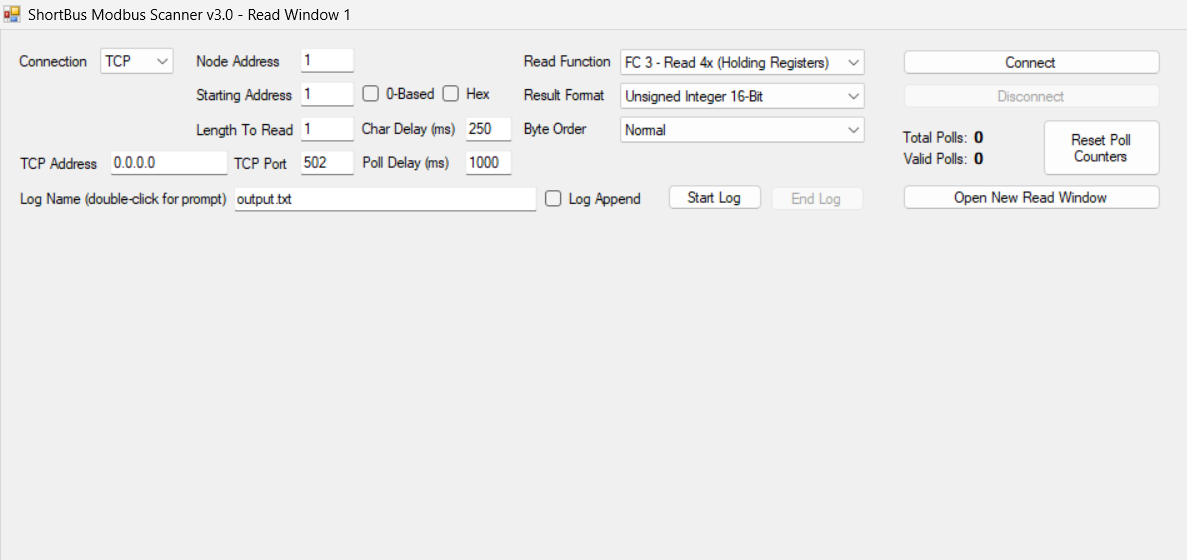
\includegraphics[width=1\linewidth]{Bilder/shortbus_fenster}
	\caption{Shortbus Desktopanwendung (ohne Inputs)} 
	\label{fig:Shortbusfenster}
\end{figure}

\subsection{Shortbus allgemeiner Teil}
Shortbus lässt sich in zwei große Bereiche gliedern. Das komplette Anzeigefenster kann in den oberen Teil (Siehe Abb.~\ref{fig:Shortbuseingabe}) und einen unteren Teil (Abb.~\ref{fig:Shortbusausgabe}) aufgeteilt werden.
Im oberen Teil von Shortbus (Abb.~\ref{fig:Shortbuseingabe}) erfolgen die gesamten Eingaben was das System (Client/Server Architektur) betrifft:
\begin{itemize}
	\item Connection: Das ist die Art, wie man sich mit dem System verbinden möchte. Man unterscheidet hierbei zwischen TCP (Transmission Control Protocol) oder COM (Schnittstelle am Laptop meist COM7)
	
	\item Node Adress: Ist die Adresse, welche vom Bauteil verwendet wird. Jedes Bauteil (\zB \gls{qbm}  oder ebm-papst) hat eine eigene Node Adresse.
	
	\item Starting Address: Diese bestimmt das erste Register, welches ausgelesen werden soll. Die Register und deren Adressen können wie folgt angegeben werden:
		\begin{itemize}
			\item ob das Register bei null anfängt (0-Based) oder nicht
			\item ob das Register in Hexadezimal (Hex) angegeben ist oder in dezimal
		\end{itemize}
	\item Length To Read: Gibt an wie viele Register ausgelesen werden (ausgelesen und angezeigt).
	\item Read Function: Hier wird die Registerart angegeben (Es gibt insgesamt 4 Registerarten).
\end{itemize}

Im unteren Teil (Abb.~\ref{fig:Shortbusausgabe}) erfolgt die Ausgabe der einzelnen \gls{modbus} Register. Dabei wird mit zuvor festgelegten Werten (Baudrate, Registerart etc.) eine Verbindung aufgebaut und die zuvor angegebene Zahl an Register wird ausgegeben. 


  
\newpage
\subsection{Shortbus Anwendung in der Entwicklungs- \ac{rltanlage}}

In der Entwicklungs- \ac{rltanlage} wird die Schnittstelle COM7 (USB-Port des Laptops) verwendet, um eine Kommunikation (Connection) mit dem \gls{modbus} aufzubauen. Welche COM Schnittstelle die richtige ist, kann im Windows Geräte-Manager nachgesehen werden. Dabei wird der \gls{modbus} per Kabel  (Abb.~\ref{fig:modbus_usbkabel}) erweitert und auf der einen Seite mit dem Laptop und dessen USB-Schnittstelle verbunden. Die andere Seite wird in der \ac{rltanlage} an den bestehenden \gls{modbus} angeschlossen. 

\begin{figure}[H]
	\centering
	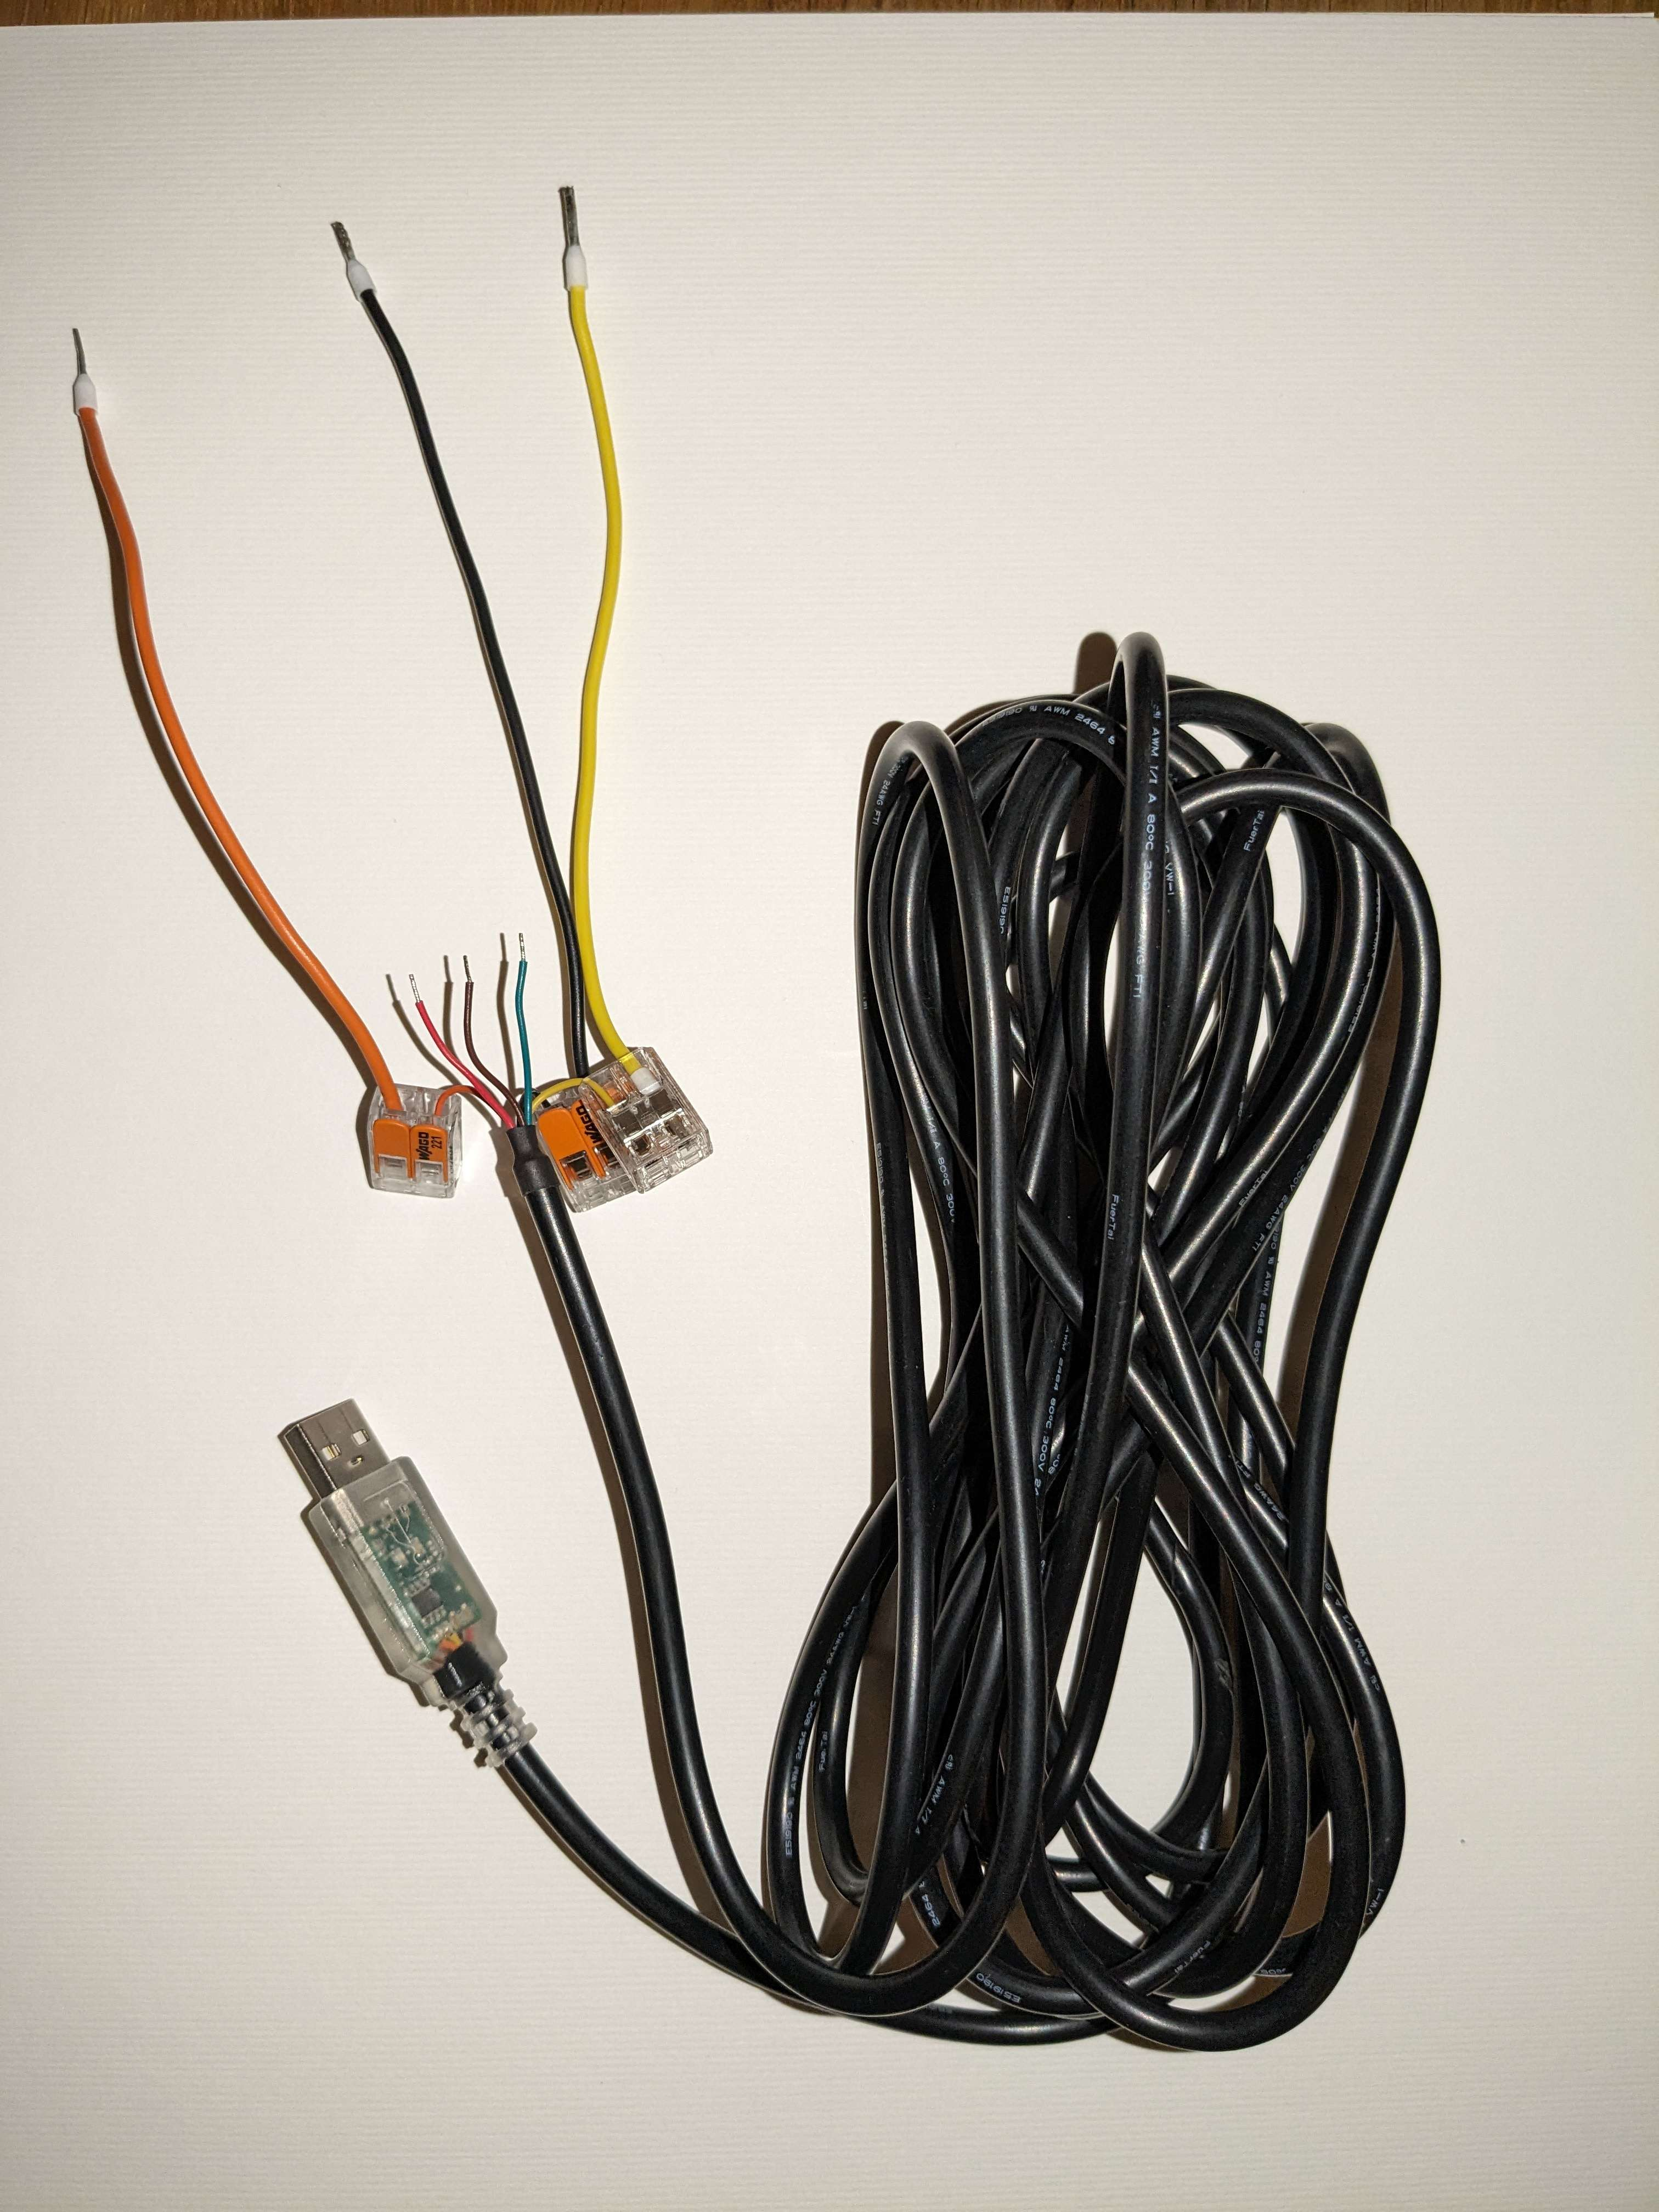
\includegraphics[width=0.3\linewidth]{Bilder/modbus_usbkabel}
	\caption{\gls{modbus} USB-Kabel} 
	\label{fig:modbus_usbkabel}
\end{figure}

Danach werden die einzelnen Komponenten (Komponenten der Entwicklungs- \ac{rltanlage}) der seriellen Kommunikation angegeben (oberer Teil des Shortbus Fensters) (Abb.~\ref{fig:Shortbuseingabe}):
\begin{itemize}
	\item Baudrate (9600)
	\item Parity (Even)
	\item Stop Bits (1)
	\item Node Adresse (2)
	\item Starting Address 1 (Register fängt bei eins an und ist in dezimal, nicht hexadezimal angegeben)
	\item Length To Read (Die ersten 85 Werte sollen ausgegeben werden)
	\item Read Funktion (FC 3 - Holding Register)
\end{itemize}

Beschreibung der Werte und Funktion von: Baudrate, Parity, Stop Bits, Read Funktion (Siehe Kapitel \ref{modbus_funktionsweise}).
Im Projekt wurde zudem die Funktion Write Multiple verwendet (Abb.~\ref{fig:writemultiple}). Diese Funktion wurde eingesetzt, um zu testen, ob das passende Register für \zB die Ventilatoren, ausgelesen wurde. Dabei wurde in das Register ein Wert eingeschrieben und getestet, ob die Ventilatoren auf einen veränderten Sollwert reagieren (sich mit vorgegebenen Sollwert Drehen). Das Gleiche gilt auch für die angesteuerten Klappen \zB WRG-Klappe (Wärmerückgewinnungsklappe). Dort wurde zum Testen dauerhaft ein Wert eingeschrieben und nachgesehen, ob sich die Klappen-Stellung ändert.

\begin{figure}[H]
	\centering
	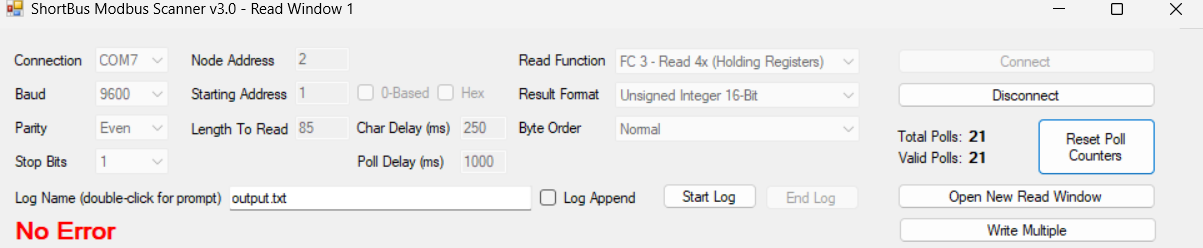
\includegraphics[width=1\linewidth]{Bilder/shortbus_eingabe}
	\caption{Shortbus Eingabefenster} 
	\label{fig:Shortbuseingabe}
\end{figure}


\begin{figure}[H]
	\centering
	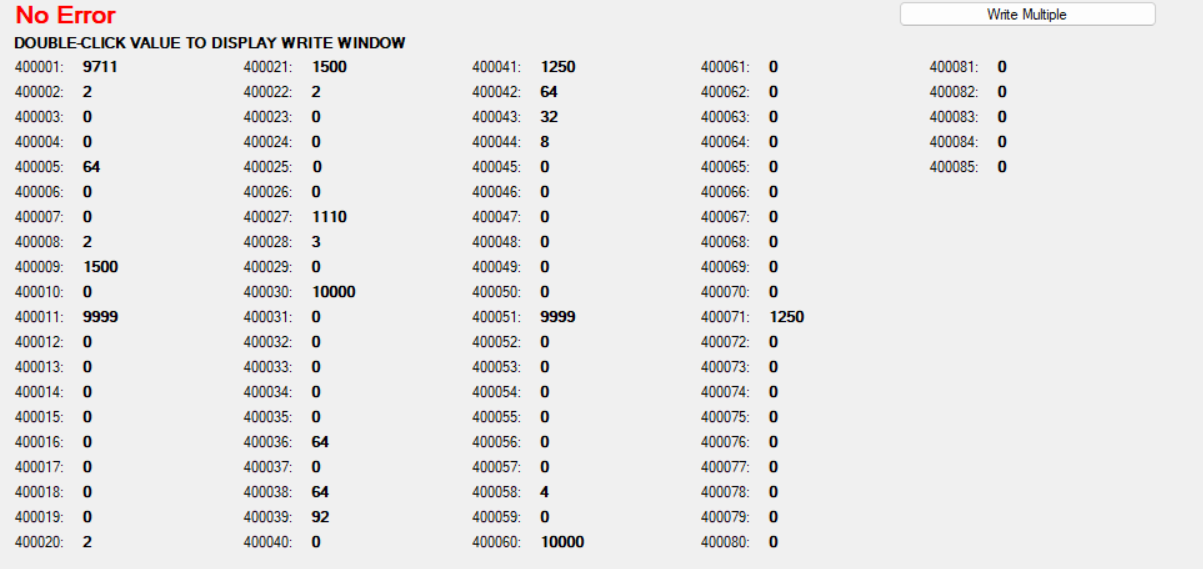
\includegraphics[width=1\linewidth]{Bilder/shortbus_ausgabe}
	\caption{Shortbus Ausgabefenster} 
	\label{fig:Shortbusausgabe}
\end{figure}

\begin{figure}[H]
	\centering
	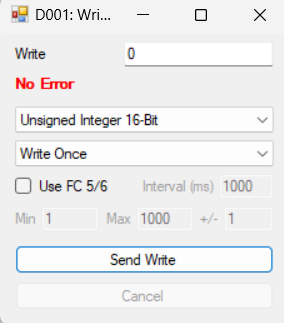
\includegraphics[width=0.3\linewidth]{Bilder/write_multiple_fenster}
	\caption{Shortbus Write Multiple Fenster} 
	\label{fig:writemultiple}
\end{figure}

\subsection{Shortbus Registerauslesung}

In der \ac{rltanlage} wurden mehrere \gls{qbm} von Siemens eingebaut. Aufgabe war es bei diesen und allen anderen Bauteilen, welche in der \ac{rltanlage} verbaut waren, die Register zu den einzelnen Werten herauszufinden um diese später in den Konfigurations-Files und für die Berechnungen bereitzustellen. 

Die ersten Versuche (Siehe  Abb.~\ref{fig:ersteauslesung}), etwas auszulesen wurden, durch einen einfachen Aufbau von einem oder zwei \gls{qbm}  bewerkstelligt. Dabei wurde herausgefunden, auf welchen Register der Druckunterschied angezeigt wird. Durch das Anschließen von Temperatursensoren konnte man überprüfen, ob auch die Register für die Analog Input Ports (Temperatur) auf die richtigen Register geschrieben wurden.

\begin{figure}[H]
	\centering
	\includegraphics[angle=90,width=0.5\linewidth]{Bilder/erste_auslesung}
	\caption{Erste Werte auslesen inkl. laufender Software} 
	\label{fig:ersteauslesung}
\end{figure}

Beschreibung der Ansteuerung anhand eines Beispiels (Abb.~\ref{fig:Shortbusausgabe}) (\gls{qbm}):
\begin{itemize}
	\item Bei diesem \gls{qbm}  kommt auf dem ersten Register die genaue Typenbezeichnung des \gls{qbm} .  
	\item Auf den Registern 5 und 7 kommen die gemessenen Druckunterschieden gemessen in Pascal(Pa) herein. 
	\item Die Register 9 und 11 sind jeweils die zwei verbauten Analog Input Ports, welche auch wiederum zwei Funktionen haben können:
	\begin{itemize}
		\item 1. Variante: Es sind Temperatursensoren (\zB Nickel1000) angeschlossen (Ausgabe in °C)
		\item 1. Variante: Es sind Klappen (\zB WRG-Klappe) angeschlossen (Ausgabe in mV)
	\end{itemize}
	\item Auf dem Register 27 und 57 sind beim \gls{qbm} die Analog Output Ports zu finden
	
	\cite[vgl.][]{siemens:2021}
\end{itemize} 
 